\documentclass{beamer}
\usepackage[utf8]{inputenc}
\usepackage[T1]{fontenc}
\usepackage[english]{babel}
\usepackage{graphicx}
\usepackage{times}

\usetheme{AGH}

\title[Realtime 4D raytracing]{Raytracing obiektów czterowymiarowych\\ w czasie rzeczywistym w języku\\Common Lisp}
\subtitle{Praca magisterska}

\author[J. Złydach]{Jacek Złydach}

\date[2013]{23.04.2013}

\institute[AGH-UST]
{Wydział Elektrotechniki, Automatyki,\\
Informatyki i Inżynierii Biomedycznej
}

\setbeamertemplate{itemize item}{$\maltese$}

\begin{document}

{
%\usebackgroundtemplate{
\includegraphics[width=\paperwidth]{titlepage}} % wersja angielska
\usebackgroundtemplate{
\includegraphics[width=\paperwidth]{titlepagepl}} % wersja polska
 \begin{frame}
   \titlepage
 \end{frame}
}

%---------------------------------------------------------------------------


\begin{frame}
\frametitle{Geometria 4D}

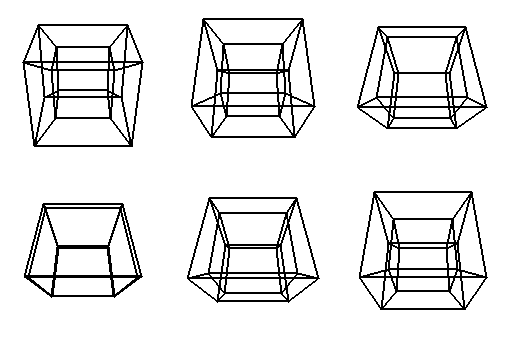
\includegraphics[scale=0.65]{hypercube-rotating.png}

\end{frame}

%---------------------------------------------------------------------------

\begin{frame}
\frametitle{Geometria 4D}

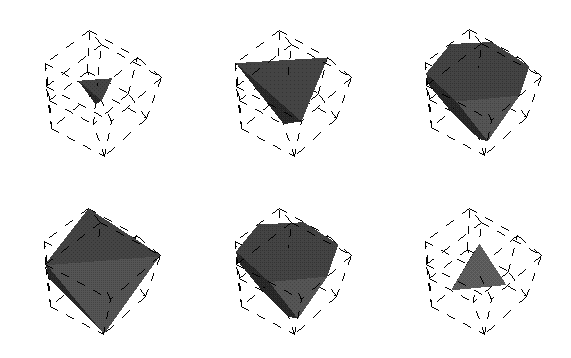
\includegraphics[scale=0.65]{hypercube-passing.png}

\end{frame}

%---------------------------------------------------------------------------

\begin{frame}
\frametitle{Raytracing}

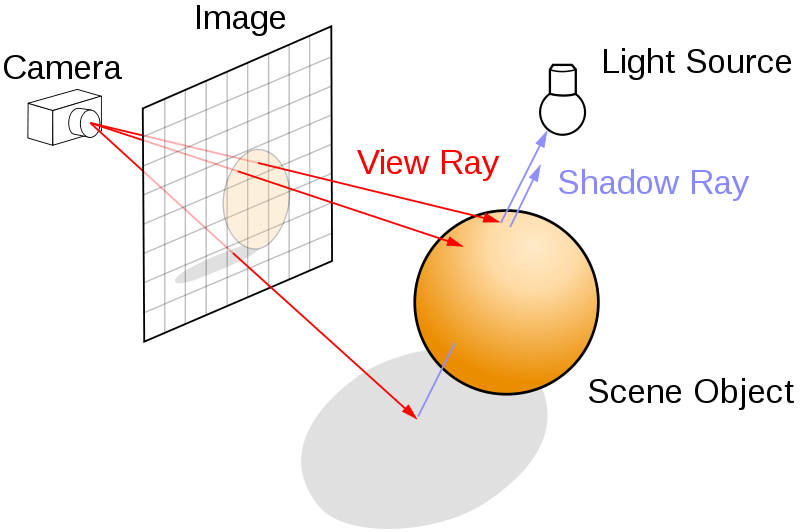
\includegraphics[scale=0.3]{raytracing.png}

\end{frame}

%---------------------------------------------------------------------------


\begin{frame}
\frametitle{Common Lisp}

\begin{itemize}
\item Wieloparadygmatowy
\item Kompilowany
\item Homoikoniczny
\item Bindingi do OpenGL
\end{itemize}

\end{frame}

%---------------------------------------------------------------------------

\begin{frame}
\frametitle{Plan prac}

\begin{itemize}
\item Kwiecień, Maj - research
\item Czerwiec+ - implementacja
\item Wrzesień/Październik (?) - obrona
\end{itemize}

\end{frame}

%---------------------------------------------------------------------------

\end{document}

